Many convex optimization methods can be interpreted as the discretization of an ordinary differential equation -- whose solution trajectories approximate the steps of the optimization algorithm. The established theory of ordinary differential equations and dynamical systems can often provide insight in the design and analysis of their corresponding discrete-time optimization algorithms. Connections between these fields have been fruitfully explored in the classical optimization literature in a number of works \cite{helmke2012optimization, schropp2000dynamical, fiori2005quasi, durr2012class, dorr2012smooth, osher2016sparse, qin2012structured, lessard2016analysis}.

In the present work we both review and advance the connection between first-order gradient methods for optimization and their continuous-time counterparts -- in particular focusing on the continuous-time limit of Nesterov's accelerated gradient method. First-order methods have regained popularity in machine learning and many other fields as data sets and problems increase in size and complexity. Thirty years ago, however, in a seminal paper Nesterov proposed a family of ``accelerated" gradient algorithm provably improving upon the convergence rate of ordinary gradient descent \cite{nesterov1983method} \footnote{Nesterov proposed two distince schemes for both accelerating gradient descent applied to both weakly and strongly convex functions -- we henceforth refer to Nesterov (I) for the scheme for weakly convex functions and Nesterov (II) for the scheme for strongly convex functions}. While these ``accelerated" methods are easy to implement, the convergence proofs of these ``accelerated" first-order gradient schemes have long been considered difficult to understand. Further, many researchers have also lacked an intuitive understanding of ``why" these methods work -- making them difficult to generalize as well.

A recent line of research initiated by \cite{su2014differential} derived, perhaps surprisingly, a \textit{second-order} ODE which is the exact limit of the \texit{first-order} Nesterov (I) scheme. Various examples and case studies related to this second-order ODE provided in \cite{su2014differential} used this conceptually simpler ODE as a tool for understanding, analyzing and generalizing Nesterov’s scheme. Since then, several researchers have attempted to both extend this work into more general settings and further understand the significance of the discretization between the continuous-time ODE perspective and the original discrete-time Nesterov schemes \cite{krichene2015accelerated, wibisono2016variational, wilson2016lyapunov}.

The purpose, structure, and contributions of this project can be broadly summarized as:
\begin{itemize}
    \item Reviewing accelerated first-order methods in both discrete and continuous time focusing on establishing the optimality lower bounds shown in \cite{nesterov2004introductory} and introducing the second-order scheme analyzed in \cite{su2014differential} for the Nesterov (I) scheme.
    \item Extending results of \cite{su2014differential} to the case of the Nesterov (II) scheme which is applicable to strongly convex functions. This includes producing both continuous-time convergence proofs for gradient descent and the Nesterov (II) scheme we derive and providing intuitive perspective connecting the Nesterov (II) scheme to the physics of the damped harmonic oscillator.
    \item Investigating the generalization of the Nesterov (I) scheme to non-Euclidean geometries -- i.e. ``accelerated" mirror descent -- studied in \cite{krichene2015accelerated}.
\end{itemize}

\subsection{Gradient Descent}

Gradient descent is an iterative optimization algorithm that can be used to minimize a function $f$ over $\mathbb{R}^{d}$. The iterates evolve as:
\begin{equation}
    x_{k+1} = x_k - s \nabla f(x_k)
\end{equation}
where $s > 0$ is the step size. 

One can provably show the convergence of gradient descent algorithm when it is used to minimize a \textit{convex} function subject to smoothness conditions on the function $f$. In particular, depending on the type of convex function we can derive different rates of convergence for its quickness in finding the global optima of $f(x)$, $x^*$. 

\begin{figure}[!h]
\begin{center}
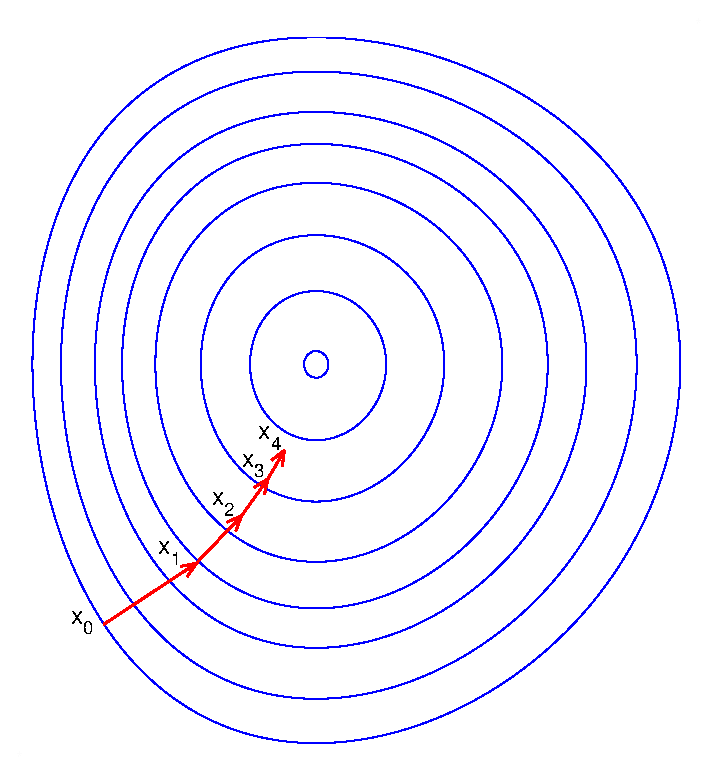
\includegraphics[width=0.2\linewidth]{SourceFiles/plots/Gradient_descent.eps}
\caption{Gradient Descent iterates moving towards the global optimum.}
\end{center}
\end{figure}

To this end, it is interesting to consider the class of functions which are restricted to being $\beta-$smooth and $\alpha-$strongly convex. 
We now recall these definitions:
\begin{definition}
If $f$ is a differentiable, convex function and $x,y$ two points in its domain, then:
\begin{equation}\label{convexity_def_eq}
f(y) \geq f(x) + \nabla f'(x)^\top (y-x)
\end{equation}
\end{definition}

\begin{definition}
$f$ is $\alpha-$strongly convex if:
\begin{equation}
f(y) \geq f(x) + \nabla f(x)^\top(y-x) + \frac{\alpha}{2} ||x - y||_2^2
\end{equation}
\end{definition}

Alternatively, a function $f$ is strongly convex if $x \rightarrow f(x) - \frac{\alpha}{2} ||x||^2$ is convex. In the case of twice differentiable functions this is equivalent to $\nabla^{2} f(x) \succeq \alpha I$. Intuitively, this is equivalent to stating that $f$ is globally \textit{lower-bounded} by a quadratic function. 

\begin{definition}
$f$ is $\beta$-smooth if:
\begin{equation}\label{fundamental_beta_eq}
f(y) \leq f(x) + \nabla f(x)^\top(y-x)+ \frac{\beta}{2} ||x - y||_2^2
\end{equation}
\end{definition}
Alternatively, a function $f(x)$ is $\beta$-smooth if its gradients $\nabla f(x)$ are $\beta-$Lipschitz:
\begin{equation}
    || \nabla f(x) - \nabla f(y) || \leq \beta ||x - y||
\end{equation}
In the case of twice differentiable functions this is equivalent to $\nabla^{2} f(x) \preceq \beta I$.
Intuitively, this is equivalent to stating that $f$ is globally \textit{upper-bounded} by a quadratic function.

If $f$ is $\alpha-$ strongly convex and $\beta-$ smooth then:
\begin{definition}
The \textbf{condition number} of $f$ is $\kappa = \frac{\beta}{\alpha}$. 
\end{definition}

\subsection{Convergence Rates}

It is well-known that gradient descent applied to a $\beta-$smooth functions achieves a $\mathcal{O}(1/k)$ convergence rate \cite{DBLP:journals/ftml/Bubeck15}:

\begin{theorem}
Let $f$ be convex and $\beta$-smooth then gradient descent with $s = \frac{1}{\beta}$ satisfies:
\begin{equation}
f(x_k) - f(x^*) \leq \frac{2\beta ||x_1 - x^* ||_2^2}{k-1}
\end{equation}
\end{theorem}

The proof of this result hinges on the use of equations \ref{fundamental_beta_eq}, \ref{convexity_def_eq} which immediately imply a bound for the minimal improvement of a single gradient descent step: $
f(x- \frac{1}{\beta} \nabla f(x) ) - f(x) \leq -\frac{1}{2\beta} ||\nabla f(x)||^2$

If the function $f$ is smooth and strongly convex the convergence rate of gradient descent is improved from $\mathcal{O}(1/t)$ to $\mathcal{O}(\exp(-t/\kappa))$ \cite{DBLP:journals/ftml/Bubeck15}:

\begin{theorem}
If $f$ is $\alpha-$strongly convex and and $\beta-$smooth then gradient descent with step size $s = \frac{2}{\alpha+\beta}$ satisfies:
\begin{equation}
f (x_{k+1}) - f(x^*) \leq \frac{\beta}{2} \exp(-\frac{4t}{\kappa+1}) ||x_1-x^*||_2^2
\end{equation}
\end{theorem}

As we will see in the next section these rates are not optimal. In fact, \cite{nesterov2004introductory} proved optimality lower bounds for the convergence rate of an first-order algorithm that can only access function and gradient evaluations. Remarkably, \cite{nesterov2004introductory} also presented an ``acceleration" scheme to achieve these lower bounds.

\begin{center}
 \begin{tabular}{||c c ||} 
 \hline
 Function Class  & Gradient Descent Convergence Rate \\ [0.5ex] 
 \hline\hline
 $\beta$-Smooth  & $\frac{1 }{k}$  \\ [1ex]
 \hline
 $\beta$-Smooth and $\alpha-$Strongly Convex   & $\exp\left(-\frac{k}{\kappa}\right)$  \\[1ex]
 \hline
\end{tabular}
\end{center}

\subsection{``Oracle" Lower bounds}

A black box optimization procedure is a mapping from the history of the algorithm to the next query point, in the algorithm's quest for the minimizer of $f$. A black-box, linear first-order optimization algorithm is any method such $x_1 = 0$ and produces the iterate $x_{k+1}$ from the values $(x_1, g_1, \cdots, x_k, g_k)$ such that $g_k \in \partial f(x_k)$ $x_{k+1} \in \text{span}(g_1, \cdots, g_k)$.  \cite{nesterov2004introductory} proved striking lower bounds showing that any black-box, linear first-order optimization algorithm could not descend a $\beta$-smooth convex function faster than at a  $\mathcal{O}(1/k^2)$ rate and a $\alpha$-strongly convex, $\beta$-smooth function faster than at a  $\mathcal{O}(\exp(-t/\sqrt{\kappa})$ rate.

In this section, we present proofs of these lower bounds for both classes of convex functions. Throughout this section we will use $e_1, \cdots, e_n$ to denote the canonical basis of $\mathbb{R}^n$, and $B_2(R) = \{ x \in \mathbb{R}^n : ||x|| \leq R\}$ the $\ell_2$-ball of radius $R$. We first show that for $\beta-$smooth convex functions there is no linear, first-order, black-box procedure achieving a faster convergence rate than $\mathcal{O}(\frac{1}{k^2})$. 

\begin{theorem}
Let $k \leq (n-1)/2 , \beta >0$, then there is a $\beta-$smooth convex function such that any black box procedure for which $x_{k+1} \in Span(g_1, \cdots, g_k)$: 

\begin{equation}
\min_{1 \leq a \leq t } f(x_a ) - f(x^*) \geq \frac{3\beta}{32} \frac{\parallel x_1 - x^*\parallel}{(k+1)^2}
\end{equation}

\end{theorem}




\proofstart


Consider the following quadratic function:

\begin{equation}
    f(x) = \frac{\beta}{8}x^T A_{2k+1}x- \frac{\beta}{4}x^Te_1
\end{equation}


Where $A_m$ is an $n\times n$ matrix defined as:

\begin{equation}
(A_m)_{i,j} = \begin{cases}
                2  &  i = i,j \leq k \\
                -1 &  j \in \{i-1, i+1\}, i \leq k, j \neq m+1\\
                0 & \text{o.w.}
            \end{cases}
\end{equation}

 
Define $f_m(x) = \frac{\beta}{8} x^T A_m x - \frac{\beta}{4}x^Te_1$ and for any function $g$ define $g^* = \min_{x \in \mathbb{R}} g(x)$.

The matrix $A_m$ satisfies the following additional properties:
\begin{itemize}
\item[1] $0 \preceq A_m \preceq 4I_n$
\item[2] $x^TA_mx = x(1)^2 + x(m)^2 + \sum_{i=1}^{m-1} (x(i)-x(i+1))^2$.
\item[3] If $y(i) = 0$ for $i \geq r$, then $y^T A_{2k+1} y = y^TA_{r}y$ and therefore by 2) $\nabla f(y) \in span(e_1, \cdots, e_{r})$. 
\item[4] The minimiser $x_m^*$ of $f_m(x)$ and its optimal value $f_m^*$ satisfy:
    \begin{align}
        x_m^*(i) = \begin{cases}
                    1-\frac{i}{m+1} & i = 1, \cdots, k \\
                    0 & \text{o.w.}
                    \end{cases}\\
        f_m^* = -\frac{\beta}{8}\left( 1-\frac{1}{m+1}\right)
    \end{align}
\end{itemize}


Notice that $x_m$ is in the span of $e_1, \cdots, e_{m-1}$.  Recall that $x_1 = 0$, and therefore that $\partial(f(x_1)) = -\frac{\beta}{4}e_1$, meaning that $x_2 \in span(e_1)$, by an inductive application of 3) we conclude that $x_m \in span(e_1, \cdots, e_{m-1})$. 

Combining the previous observations we conclude the following string of inequalities:


\begin{equation}
f(x_m) - f^* = f_s(x_m) - f_{2k+1}^* \geq f_m^* - f^*_{2k+1} \geq f_k^* - f_{2k+1}^*
\end{equation}

Since $\parallel x_m^* \parallel^2 = \sum_{i=1}^m \left( \frac{i}{m+1}\right)^2 \leq \frac{m+1}{3}$ we obtain:

\begin{equation}
f_k^* - f_{2k+1}^* =\frac{\beta}{8}\left( \frac{1}{k+1} - \frac{1}{2k+2}\right) \geq \frac{3\beta}{32} \frac{\parallel x_{2k+1}*\parallel^2}{(k+1)^2}
\end{equation}

This concludes the proof. 

\proofend









\begin{theorem}
If the condition number $\kappa > 1$, then there is a $\beta-$smooth and $\alpha-$strongly convex function $f: l_2 \rightarrow \mathbb{R}$ with $\kappa = \frac{\beta}{\alpha}$ such that for any $k \geq 1$ and any black box procedure for which $x_{m+1} \in Span( g_1, \cdots, g_m)$:

\begin{equation}
f(x_k) - f(x^*) \geq \frac{\alpha}{2} \left(\frac{ \sqrt{\kappa}-1}{\sqrt{\kappa}+1}\right)^{2(k-1)} \parallel x_1 - x^* \parallel^2
\end{equation}

When $\kappa$ is large, $\left(\frac{ \sqrt{\kappa}-1}{\sqrt{\kappa}+1}\right)^{2(t-1)} \parallel x_1 - x^* \parallel^2 \approx \exp( -\frac{4(t-1)}{\sqrt{\kappa}})$


\end{theorem}

\proofstart

The main ideas of this proof are very similar to those used in the previous one. Denote by $A$ the infinite dimensional linear operator corresponding to an inifinite matrix with $2$ in the diagonal, and $-1$ on the upper and lower diagonals. This operator is a generalization of the finite dimensional $A_m$ operators found in the previous section. 

We will show that the following $\alpha-$convex and $\beta-$smooth function:

\begin{equation}
f(x) = \frac{\alpha(\kappa-1)}{8} \left( \langle Ax, x \rangle - 2\langle e_1, x \rangle \right) + \frac{\alpha}{2} \parallel x \parallel^2
\end{equation}


Since $f$ is $\alpha-$strongly convex $f(x_m) - f(x^*) \geq \frac{\alpha}{2}\parallel x_m - x^*\parallel^2$. Therefore it only remains to lower bound $\parallel x_m - x^*\parallel^2$.

$A$ has similar properties to its finite version, namely $0 \preceq A \preceq 4I$ and $x_k(i) =0 \forall i \geq k$. The later immediately implies that: 

\begin{equation}
\parallel x_k - x^* \parallel^2 \geq \sum_{i=k}^\infty x^*(i)^2
\end{equation}

To instantiate the lower bound we compute $x^*$. After differentiating and setting the gradient to zero we find the optimum is achieved by $x^*$ satisfying:

\begin{equation}
x^*(i) = \left( \frac{\sqrt{\kappa} - 1}{\sqrt{\kappa} +1} \right)^i 
\end{equation}

Putting all these bound together:

\begin{equation}
f(x_k) - f(x^*) \geq \frac{\alpha}{2}\sum_{i=k}^\infty \left( \frac{\sqrt{\kappa} - 1}{\sqrt{\kappa} +1} \right)^{2i} 
\end{equation}

Recall that $x_1 =0$. The geometric sum can be rewritten as 
\begin{equation}
\left( \frac{\sqrt{\kappa} - 1}{\sqrt{\kappa} +1} \right)^{2(k-1)} \left( \sum_{i=1}^\infty \left( \frac{\sqrt{\kappa} - 1}{\sqrt{\kappa} +1} \right)^{2i} \right) = \left( \frac{\sqrt{\kappa} - 1}{\sqrt{\kappa} +1} \right)^{2(k-1)} \parallel x_1 - x^* \parallel^2
\end{equation}

This concludes the proof.

\proofend

The following table sumarizes the lower bounds above and the gradient descent rates. 

\begin{center}


 \begin{tabular}{||c c c ||} 
 \hline
 Function Class   & GD  & Lower bound \\ [0.5ex] 
 \hline\hline
 $\beta$-Smooth & $\frac{1}{k}$ &  $\frac{1}{k^2}$\\ [1ex]
 \hline
 $\beta$-Smooth, $\alpha-$Strongly Convex  &  $\exp\left(-\frac{k}{\kappa}\right)$ &  $\exp\left(-\frac{k}{\sqrt{\kappa}}  \right)$ \\ [1ex]
 \hline
\end{tabular}



\end{center}

